
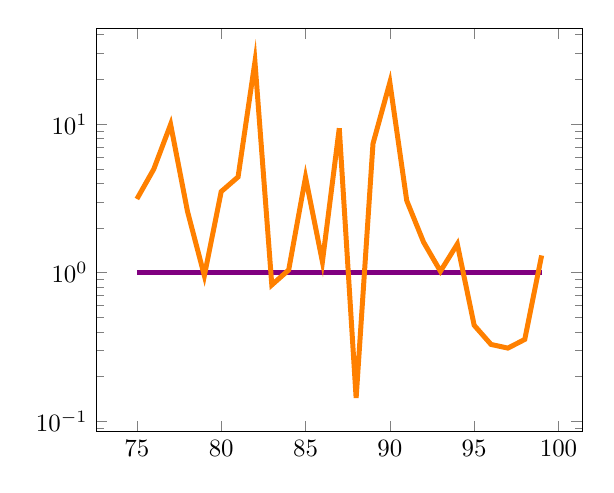
\begin{tikzpicture}[scale=0.9]
\begin{semilogyaxis}
\addplot[color=violet,line width=2pt] coordinates {(75,1.0)(76,1.0)(77,1.0)(78,1.0)(79,1.0)(80,1.0)(81,1.0)(82,1.0)(83,1.0)(84,1.0)(85,1.0)(86,1.0)(87,1.0)(88,1.0)(89,1.0)(90,1.0)(91,1.0)(92,1.0)(93,1.0)(94,1.0)(95,1.0)(96,1.0)(97,1.0)(98,1.0)(99,1.0)};
\addplot[color=orange,line width=2pt] coordinates {(75,3.134589932549902)(76,4.975734687155631)(77,9.955987006155498)(78,2.586621907047667)(79,0.9550081679103243)(80,3.515639296578849)(81,4.411265230327821)(82,26.26157295781638)(83,0.8275868661988794)(84,1.0428536886171644)(85,4.390292161810932)(86,1.184829292518715)(87,9.373411322366767)(88,0.14346178496278622)(89,7.387117386643939)(90,19.06352324180824)(91,3.0588568431723764)(92,1.6047979872369205)(93,1.0230274402088197)(94,1.5582949419359302)(95,0.4428517967530336)(96,0.32908056902508415)(97,0.31091982788674066)(98,0.35572141329395085)(99,1.3066858578257803)};

\end{semilogyaxis}
\end{tikzpicture}
